\documentclass[12pt]{article}
\usepackage{graphicx}
\graphicspath{{figures/}}
\usepackage{amsmath}
\usepackage{amsthm}
\usepackage{newtx}

\usepackage{framed} 
\usepackage[margin=1in]{geometry}

\newtheorem{prop}{Proposition}

\begin{document}
\begin{center}
  \large
  Deleting Vertices and Relations in the \texttt{Posets} Julia Package
\end{center}

\noindent{\textbf{Deleting Vertices}}

Deleting vertices from a poset is somewhat different from deleting
vertices in a graph. When a vertex is deleted from a graph, the vertex
and all edges incident with that vertex are removed. Similarly, when
a vertex is removed from a poset, the relations between all the
remaining vertices remain unchanged. However, this is not the same as
simply deleting a vertex and its edges from the poset's Hasse
diagram. 

Consider the poset on the left in Figure~\ref{fig:vertex-deletion}. 
Mathematically, deleting vertex $2$ from this poset results in the
poset in the middle of the figure. In the Hasse diagram we have an
edge from 1 upward to 3 because $1\prec 3$ in the original poset, and
so we still have $1 \prec 3$ after the deletion. Similarly, the
relation $4\prec3$ is preserved.

\begin{figure}[h]
\begin{framed}
  \begin{center}
    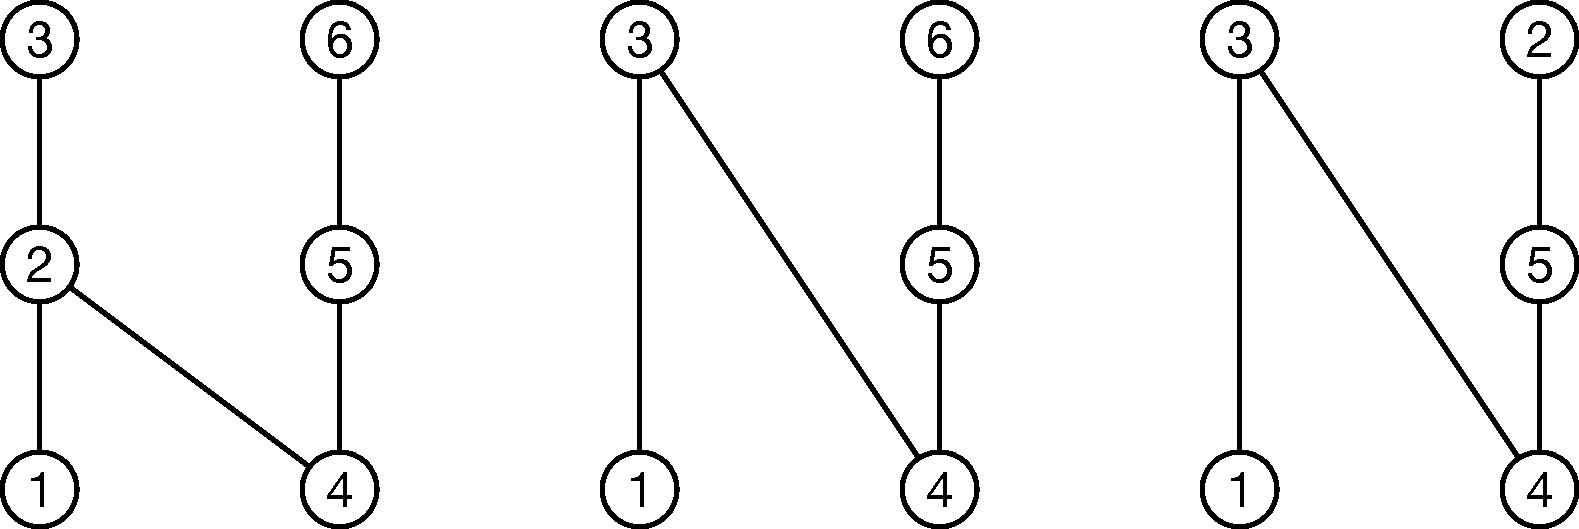
\includegraphics[scale=0.3]{vertex-deletion}
  \end{center}
  \caption{Vertex deletion in \texttt{Posets}. When vertex $2$ is
    deleted from the poset on the left, mathematically we have the
    poset in the middle.  However, following \texttt{Graphs}'
    convention, vertex $6$ is renamed by the deleted vertex, $2$,
    giving the result on the right.}
  \label{fig:vertex-deletion}
\end{framed}
\end{figure}

However, the Julia \texttt{Posets} package is based on the
\texttt{Graphs} package. A key convention of graphs (and hence of
posets) in these packages is that the vertex set is always of the form
$\{1,2,\ldots,n\}$. If vertex $n$ is deleted, no special action needs
to be taken. But if a vertex $k$ (with $k<n$) is removed, then the
name $n$ is no longer valid by the naming convention. In this case,
the vertex formally named $n$ is renamed $k$ (the label of the deleted
vertex). As a result, the result in \texttt{Posets} of deleting vertex
$2$ in Figure~\ref{fig:vertex-deletion} is the poset on the right.

This is illustrated in Julia as follows:
\begin{verbatim}
julia> p = chain(3) + chain(3);
julia> add_relation!(p, 4, 2);
julia> rem_vertex!(p, 2);
julia> collect(relations(p))
5-element Vector{Relation{Int64}}:
 Relation 1 < 3
 Relation 4 < 2
 Relation 4 < 3
 Relation 4 < 5
 Relation 5 < 2
\end{verbatim}

\newpage
\noindent{\textbf{Deleting Relations}}

Deleting a relation from a poset is complicated. The simplest case is
the removal of a relation $a \prec b$ where $b$ is a cover of $a$. In
this case, it is possible just to remove the single relation $a \prec
b$ and make no other changes to the poset. This is illustrated in
Figure~\ref{fig:cover-edge-deletion} in which we delete the cover
relation $2\prec$ from the linear order $1\prec2\prec3\prec4$. 
\begin{figure}[h]
  \begin{framed}
    \begin{center}
      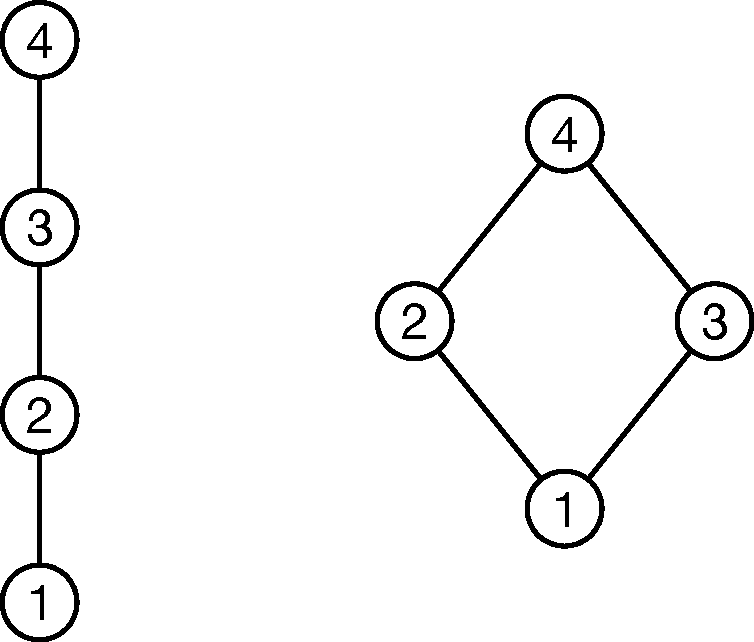
\includegraphics[scale=0.3]{cover-edge-deletion}
    \end{center}
    \caption{Deleting a cover relation, $2\prec3$, from a poset.}
    \label{fig:cover-edge-deletion}
  \end{framed}
\end{figure}

The following Julia code implements the action of deleting $2 \prec 3$
from a 4-element chain:
\begin{verbatim}
julia> p = chain(4);
julia> rem_relation!(p, 2, 3);
julia> collect(relations(p))
6-element Vector{Relation{Int64}}:
 Relation 1 < 2
 Relation 1 < 3
 Relation 1 < 4
 Relation 2 < 3
 Relation 2 < 4
 Relation 3 < 4
\end{verbatim}
That this yields a partial order follows from
Proposition~\ref{prop:ab}. 

The situation is different for non-cover relations. For example,
consider the linear order $1\prec2\prec3\prec4\prec5$. Suppose we
wish to delete the relation $2\prec4$. If we only delete that one
relation, we would still have $2\prec3$ and $3\prec4$, so omitting
$2\prec4$ would result in a violation of transitivity. 

More generally, suppose we wish to remove the relation $a\prec b$ from
a poset. If there is an element $x$ with $a\prec x\prec b$ we cannot
delete just $a\prec b$ and keep both $a \prec x$ and $x\prec b$. There
is no \emph{a priori} reason to prefer one of $a\prec x$ or $x \prec
b$ for deletion (or retention). Hence, it is a design decision that
when removing a relation $a \prec b$ we also remove both relations $a
\prec x$ and $x \prec b$ for all $x$ between $a$ and
$b$. Proposition~\ref{prop:ab} ensures that the new relation gives a
partial order. 

For example, suppose we wish to delete the relation $2\prec4$ from the
linear order $1 \prec 2 \prec 3 \prec 4 \prec 5$. Our implementation
deletes not only $2\prec 4$ but also $2\prec3$ and $3\prec4$ as well. 
This is illustrated in Figure~\ref{fig:other-edge-deletion}. 
\begin{figure}[h]
  \begin{framed}
    \begin{center}
      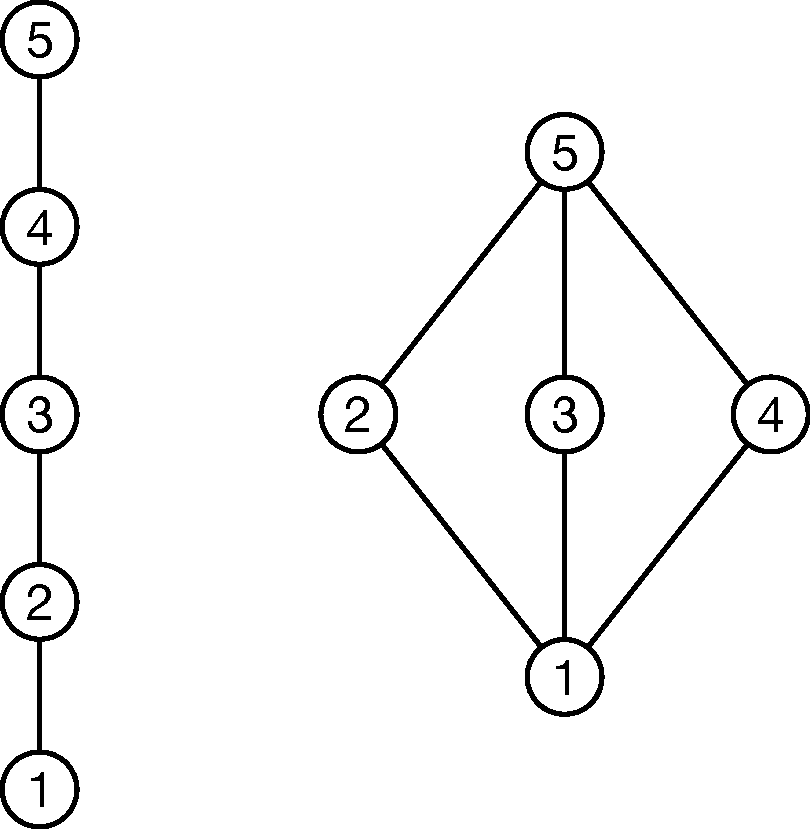
\includegraphics[scale=0.3]{other-edge-deletion}
    \end{center}
    \caption{Deleting the non-cover relation $2\prec4$ from the poset
      on the left yields the poset on the right.  The function
      \texttt{rem\_relation!(p,a,b)} not only deletes $a\prec b$, but
      also all relations of the form $a\prec x$ and $x\prec b$ for
      vertices $x$ between $a$ and $b$.}
    \label{fig:other-edge-deletion}
  \end{framed}
\end{figure}

This Julia code illustrates the deletion:
\begin{verbatim}
julia> p = chain(5);
julia> rem_relation!(p, 2, 4);
julia> collect(relations(p))
7-element Vector{Relation{Int64}}:
 Relation 1 < 2
 Relation 1 < 3
 Relation 1 < 4
 Relation 1 < 5
 Relation 2 < 5
 Relation 3 < 5
 Relation 4 < 5
\end{verbatim}

Note on notation: $[a,b] = \{ c \in V \colon a \preceq c \preceq b
\}$. 

\begin{prop}\label{prop:ab}
  Let $P=(V,\prec)$ be a poset. Let $a,b\in V$ with $a \prec b$.
  Let $\prec'$ be a new relation on $V$ in which $x\prec'y$ provided
  $x\prec y$ and neither $x=a \prec y \preceq b$ nor 
  $a\preceq x \prec y=b$.

  Then $(V,\prec')$ is a partially ordered set.
\end{prop}


\begin{proof}
  Note that if $x\prec' y$ then necessarily $x \prec y$. [Formally,
  ${\prec'} \subseteq {\prec}$.]

  We cannot have $x \prec' x$ because that would imply $x \prec
  x$. Likewise, we cannot have $x \prec' y$ and $y\prec' x$ as that
  would imply $x\prec y$ and $y\prec x$. Hence $\prec'$ is irreflexive
  and antisymmetric. We need to prove that $\prec'$ is transitive.

  Suppose $x \prec' y \prec' z$. We must show $x \prec' z$. Note that
  this supposition implies $x \prec y \prec z$ and hence $x \prec
  z$. To show that $x \prec' z$ we need to rule out both $x=a\prec
  z\preceq b$ and $a\preceq x \prec b=z$.
    
  Suppose $x=a\prec z\preceq b$. Since $y$ is between $x$ and $z$, we
  have $x=a \prec y \prec z \preceq b$ implying that $x=a\not\prec'y$,
  a contradiction.

  Supposing $a\preceq x \prec b=z$ leads to a similar contradiction.

  Therefore $x \prec' z$ and we conclude that $\prec'$ is transitive
  and that $(V,\prec')$ is a partially ordered set.
\end{proof}

\end{document}